\documentclass[a4paper]{article}

\usepackage[english]{babel}
\usepackage[UKenglish]{isodate}
\usepackage[parfill]{parskip}
\usepackage{float}
\usepackage{graphicx}
\usepackage{booktabs}
\usepackage{csquotes}
\usepackage{listings}
\usepackage[margin=2.5cm]{geometry}
\usepackage{color}
\usepackage{tikz}
\usepackage{siunitx}
\usetikzlibrary{shapes.geometric, arrows}

\renewcommand{\lstlistingname}{Algorithm}% Listing -> Algorithm
\renewcommand{\lstlistlistingname}{List of \lstlistingname s}
\newcommand{\nth}{\textsuperscript}

\tikzstyle{startstop} = [rectangle, rounded corners, minimum width=4cm, minimum height=1cm,text centered, draw=black]
\tikzstyle{process} = [rectangle, minimum width=4cm, minimum height=1cm, text centered, draw=black]
\tikzstyle{decision} = [diamond, minimum width=4cm, minimum height=1cm, text centered, draw=black]
\tikzstyle{arrow} = [thick,->,>=stealth]
\tikzstyle{line} = [thick, -]

\definecolor{backcolour}{rgb}{0.95,0.95,0.92}

\lstdefinestyle{mystyle}{
	backgroundcolor=\color{backcolour},   
	basicstyle=\footnotesize,
	breakatwhitespace=false,		 
	breaklines=true,				 
	captionpos=t,					
	keepspaces=true,				 
	showspaces=false,				
	showstringspaces=false,
	showtabs=false,				  
	tabsize=4
}
 
\lstset{style=mystyle}

\title{\vspace{2cm}COMP2121 Project - Design Manual}
\author{Kevin Zihong Ni \& Phoebe Zhou\\\small\texttt{z5025098 z5088051}}

\begin{document}

\newgeometry{margin=1.5in}
\maketitle
\vspace{2cm}
\tableofcontents
\pagebreak
\restoregeometry

\section{System Flow Control} \label{sec:sfc}
\begin{center}
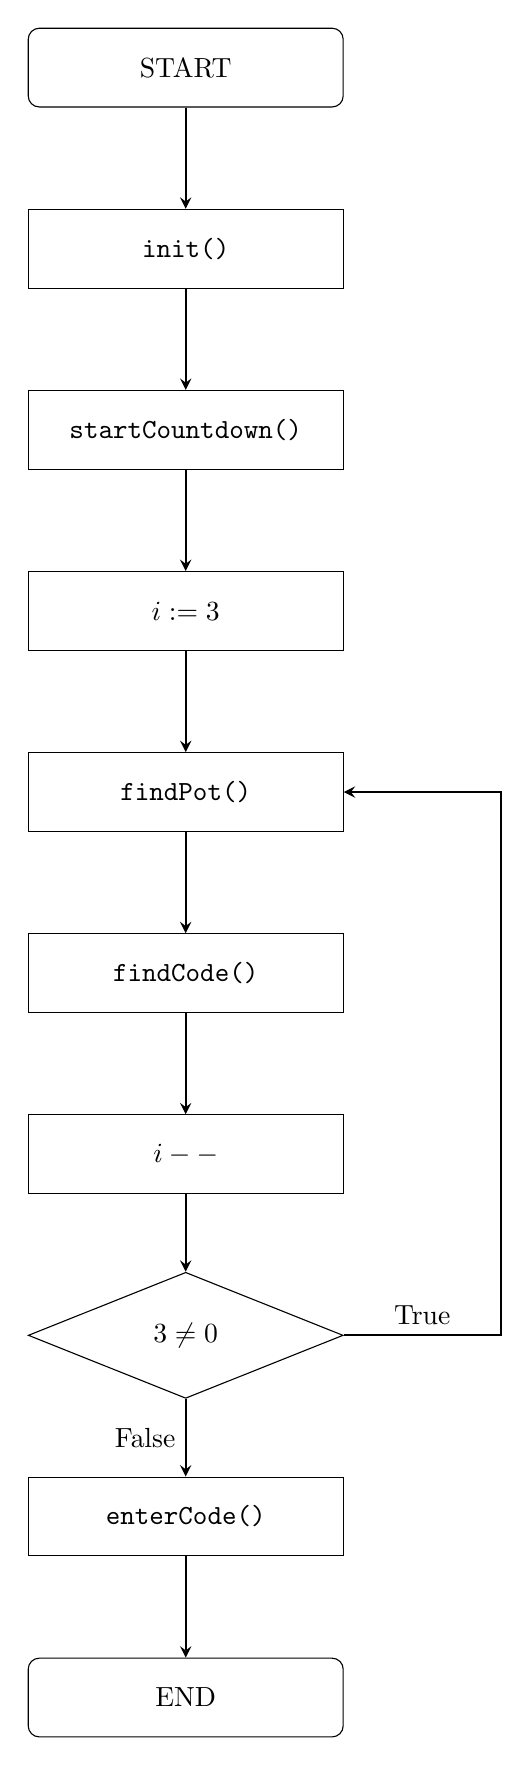
\begin{tikzpicture}[node distance=2.3cm]

	\node (start) [startstop] {START};
	\node (init) [process, below of=start] {\verb|init()|};
	\node (stcd) [process, below of=init] {\verb|startCountdown()|};
	\node (seti) [process, below of=stcd] {$i := 3$};
	\node (pot) [process, below of=seti] {\verb|findPot()|};
	\node (find) [process, below of=pot] {\verb|findCode()|};
	\node (dec) [process, below of=find] {$i--$};
	\node (loop) [decision, below of=dec] {$3 \neq 0$};
	\node (enter) [process, below of=loop] {\verb|enterCode()|};
	\node (end) [startstop, below of=enter] {END};

	\draw [arrow] (start) -- (init);
	\draw [arrow] (init) -- (stcd);
	\draw [arrow] (stcd) -- (seti);
	\draw [arrow] (seti) -- (pot);
	\draw [arrow] (pot) -- (find);
	\draw [arrow] (find) -- (dec);
	\draw [arrow] (dec) -- (loop);
	\draw [arrow] (loop) -- node[anchor=east] {False} (enter);
	\draw [arrow] (loop) -- node[anchor=south] {True} +(4, 0) |- (pot);
	\draw [arrow] (enter) -- (end);

\end{tikzpicture}
\end{center}

\section{Data Structures Dictionary}

\begin{table}[H]
\centering
%\caption{Data Structures Dictionary}
\label{tbl:dict}
\begin{tabular}{@{}lllp{9cm}@{}}
\toprule
Variable Name & Data Type        & Bytes & Description \\ \midrule
\multicolumn{4}{l}{Global Variables} \\ \midrule
fours         & unsigned integer & 1     & Count used by Timer 4 to calculate a second (each count represents 1/30th of a second) \\
bounce        & unsigned integer & 1     & Counter used for debouncing PB1 \\
seed          & unsigned integer & 2     & Seed used for random number generation \\
roundsleft    & unsigned integer & 1     & How many rounds are left in the game \\
at            & enumeration      & 1     & Which round the player is in \\
ocount        & unsigned integer & 1     & Stores the number of seconds per potentiometer round \\ \midrule
\multicolumn{4}{l}{Potentiometer Variables} \\ \midrule
wadc          & flag             & 1     & Stores whether or not the system is waiting on an ADC reading \\
count         & unsigned integer & 1     & Stores the number of seconds left in the last pot round \\
adcreading	& unsigned integer	& 2 & Stores the most recent ADC reading \\  
potwin		& unsigned integer	& 2	& Counter to count 1 second to win the potentiometer round \\ 
temp4:temp3	& unsigned integer	& 2	& Target potentiometer value for the current round \\

\bottomrule
\end{tabular}
\end{table}

\section{Algorithm Descriptions}

The main algorithms used in the program are as follows (shown in C code).

\subsection{Algorithm for \texttt{startCountdown}}
\begin{lstlisting}[language=C]

int cdTimer;

void startCountdown() {

	cdTimer = '4';
	do {
		cdTimer--;
		display(cdTimer);
		
		buzzerOn();
		waitms(245);
		buzzerOff();
		waitms(750);
	} while(cdTimer >= '2');
	return;
}		

\end{lstlisting}

\subsection{Algorithm for \texttt{findPot}}
\begin{lstlisting}[language=C]

#define IN_POT 2

int seed;
int second;
int count;
int at;
int adcreading;
int potwin;
int wadc;

void timerInterrupt { // timer with a frequency of 32Hz
	if(at == IN_POT){
		if(potwin){
			//increment win countdown
			potwin++;
		}
		if(second == 30) {
			//decrement coundown, check lose condition
			second = 0;
			count--;
			if(!count) {
				lose();
			}
			display(count);

			//turn on the buzzer
			buzzeron();
		} else if(((count == ocount) && (second == 30 >> 1)) || ((count != ocount) && (second == 30 >> 2))) {

			//turn off the buzzer
			buzzeroff();				
		} else if(second & 0b11 == 0 && !wadc) {

			//read from adc
			wadc = 1;
			startReadFromAdc();
		}
	}
	second++;
	return;
}

void resetPot() {
	while(adcreading);
	return;
}

void findPot() {

	at = IN_POT;
	int target = seed; // random number
	target &= 0x3FF;
	reset:
	resetPot();
	while(1) {
		if(adcreading > target) {
			goto reset;
		}
		if(target - adcreading < 48){
			PORTC = 0xff;
		} else {
			PORTC = 0;
		}
		if(target - adcreading < 32){
			PORTG = 0b1;
		} else {
			PORTG = 0;
		}
		if(target - adcreading < 16){

			PORTG = 0b11;
			if(!adcreading) adcreading++;
			if(potwin >= 31) break;
		} else {

			PORTG &= ~0b10;
			potwin = 0;
		}
	}
}

\end{lstlisting}

\section{Module Specifications}

\subsection{Initialisation (\texttt{Init})}

This module is jumped to from the RESET vector and as of a result, is always the first function that
is run when the board is powered on or reset from the game complete screen or a PB0 button press. It resets all 
of the general purpose and I/O registers to their starting values. This is especially important when a reset 
from a game complete screen or PB0 button press occurs as in those cases, not all of the memory will be reset to 
zero for free. This module is also responsible for the generation of the random seed by incrementing that
variable until the button PB1 is first pressed.

This module takes in the keypad buttons; A, B, C and D, as input. These buttons change the difficulty of the
program by changing the variable ocount which is later used in the program to determine the time allowed for 
the player to find the potentiometer position. The module prints out the lines, "\texttt{2121 16s1 Safe Cracker}", to the screen as output.


\subsection{Find Potentiometer Position (\texttt{findPot})}
This module is called 3 times throughout the duration of the game as shown in section \ref{sec:sfc}. It uses the
Analog to Digital converter to determine the position of the pot and it changes the state of the LED bar as
output to display the proximity of the current position to the target one. The module also uses a timer to count
down from a value determined in the Initialisation module and displays it to the LCD screen. Lastly, the module
uses the buzzer module to create a beep for a quarter of a second whenever the timer counts down.

\subsection{Find Code (\texttt{findCode})}
This module is called directly after the \verb|findPot| module. Using the seed, It generates 3 random keys and 
stores them in memory on the first time it is called. From there it uses the keyboard module as input to search
for any keys that the user is pressing. It provides output in the form of providing power to the motor to
create feedback to the user when the correct key is held down. It uses a timer to determine the duration of
the key being held down in order to decide whether or not to proceed through the game.

\subsection{Enter Code (\texttt{enterCode})}
The module is similar to the Find Code module in that it takes in input through the keypad. However, instead of
providing output to a motor as feedback, it instead prints asterisks to the LCD screen. It also takes in the
random keys generated by \verb|findCode| as input as the module's purpose is to prompt the user for the keys
that they found in \verb|findCode|.

\subsection{Analog to Digital Converter}
The ADC module uses the the function \verb|startAdcRead| and the interrupt function \verb|adcread| as its 
interface. The former initiates an AdcRead and is called by a timer periodically (at a frequency of 
\SI{8}{\hertz}) during the "Find POT position" part of the game. The latter actually reads the value from the 
board's ADC and stores it in the variable \verb|adcreading| as output to be used by the \verb|findPot| module.

\subsection{LCD display}
This module takes in either immediate values or values in a register and communicates to the LCD display to
display them as their ASCII symbols. It is also capable of taking in a register and displaying it as its
hindu-arabic numeral representation by first converting the value from binary to decimal and then displaying
the appropriate digits one by one.

\subsection{Buzzer}
The buzzer module uses a dedicated timer to control the output waveform to the pin connected to
the buzzer. The buzzer could then be turned on and off respectively by either setting or clearing the interrupt
mask for that timer. This was abstracted by using two functions \verb|buzzeron| and \verb|buzzeroff| which were
called by the rest of the program to control the buzzer.

\subsection{Keyboard}
The keyboard module takes in input from the keypad and debounces the keypad by waiting until the key has been
lifted. It reads the input from the keypad by repeatedly polling the relevant pins and returns any output 
in the temp register. This module is used in the \verb|findKey| and \verb|enterKey| modules to determine which 
key is being entered by the player.


\end{document}
